\documentclass[a4paper,11pt]{article} % Cambiato da 12pt a 11pt
\usepackage[utf8]{inputenc}
\usepackage[italian]{babel}
\usepackage{amsmath,amsfonts,amssymb,amsthm}
\usepackage{graphicx}
\usepackage{fancyhdr}
\usepackage{geometry}
\usepackage{titlesec}
\usepackage{mathtools}
\usepackage{caption}
\usepackage{amssymb}
\usepackage{bbm}
\usepackage{fancyhdr}
\usepackage{xcolor}
\usepackage{subcaption}
\usepackage{enumitem}
\definecolor{TODO}{HTML}{65fe08}

%funzioni mie
\newcommand{\pgraf}[1]{\left\{ #1 \right\}}
\newcommand{\pquad}[1]{\left[ #1 \right]}
\newcommand{\ptond}[1]{\left( #1 \right)}

% Impostazioni di pagina
\geometry{margin=1in}
\pagestyle{fancy}
\fancyhf{}
\rfoot{\thepage}
\rhead{\thepage}
\lhead{\leftmark}
\setlength{\headheight}{15pt}
\renewcommand{\headrulewidth}{0.4pt}
\renewcommand{\footrulewidth}{0pt}


% Impostazioni per i titoli delle sezioni
\titleformat{\section}[block]{\normalfont\large\bfseries}{\thesection}{1em}{} % Cambiato da \Large a \large
\titleformat{\subsection}[block]{\normalfont\normalsize\bfseries}{\thesubsection}{1em}{} % Cambiato da \large a \normalsize
\titleformat{\subsubsection}[block]{\normalfont\normalsize\bfseries}{\thesubsubsection}{1em}{} % Cambiato da \normalsize a \small
\parindent 0px 		

% Inizia il documento
\begin{document}

% Pagina del titolo
\title{\textbf{Riassunto P.P.M. // Corso di Progettazione e Produzione Multimediale}}
\author{Francesco Gori \and Elisa Farri}
\date{\today}
\maketitle

% Intestazione personalizzata per il frontespizio
\thispagestyle{fancy}
\lhead{}
\rhead{Riassunto P.P.M.}

% Indice
\tableofcontents

% Inizia il contenuto del documento
\newpage

\section{Immagini Digitali}
Le immagini digitali sono istantanee elettroniche di una scena o scansionate da documenti, come fotografie, manoscritti, testi stampati e opere d'arte. \\
Esse vengono campionate e mappate come griglie di pixel, a ciascuno dei quali viene associato un valore tonale in codice binario (nero, bianco, scala di grigi o di colore).\\
I bit di ogni pixel vengono memorizzati da un computer e sono spesso compressi con rappresentazioni matematiche.\\

\subsection{Profondità di Bit (bit depth)}
La profondità di bit è determinata dal numero di bit utilizzati per definire ciascun pixel, ad esempio:
\begin{itemize}
\item Un'immagine bitonale è composta da pixel costituiti da 1 bit ciascuno (tipicamente bianco o nero)
\item Un'immagine in scala di grigi è composta da pixel rappresentati ciascuno da più bit di informazione (in genere da 2 a 8, o anche più) 
\item Un'immagine a colori è tipicamente rappresentata con una bit depth tra 8 e 24 o più
\end{itemize}

\subsection{Formazione dell'Immagine a Colori}
La formazione dell'immagine a colori è determinata dalla distribuzione della potenza radiante della luce incidente, dalla riflessione dei materiali e dalle caratteristiche della telecamera.

\subsection{Fotocamere Digitali RGB}
\begin{minipage}{0.6\textwidth}
Le immagini digitali sono oggi ottenute da fotocamere digitali che usano sensori CMOS o CCD per acquisire tre segnali nelle lunghezze d'onda del rosso (R), del verde (G) e del blu (B).

Il motivo per questa scelta viene dalla volontà di imitare il comportamento dei recettori presenti negli occhi umani.

Lo spettro della luce riflessa può essere quindi rappresentato con un vettore di 3 elementi, che rappresentano le proporzioni dei colori primari rosso, verde e blu utilizzati per produrlo. Questi valori vengono detti "Tristimolo", quindi: $ RGB_{values}=Colour*Tristimulus $
\end{minipage}
\begin{minipage}{0.4\textwidth}
    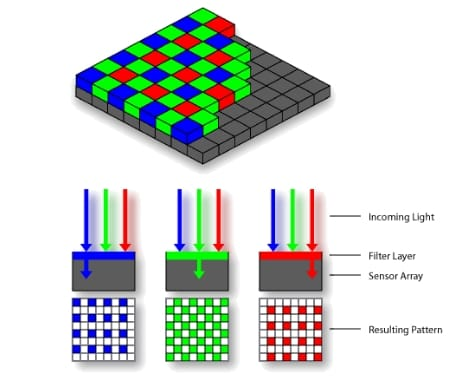
\includegraphics[width=\textwidth]{BayerPatternRGB}
\end{minipage}

Nelle fotocamere digitali i recettori RGB vengono spesso disposti in un Filtro Bayer: al verde vengono assegnati il doppio di recettori rispetto al rosso e al blu, in modo da favorire la luminosità dell'immagine. 

\subsection{Algoritmi di Demosaicizzazione}
Dato che su ogni singolo pixel viene originariamente salvato solo un colore su tre, non si può determinare a priori il colore della luce riflessa. Per questo motivo, sono stati introdotti degli algoritmi che stimano per ciascun pixel i livelli dei colori mancanti. Questi algoritmi di Demosaicizzazione vanno infatti a calcolare un valore verosimile per gli altri colori in base a quelli presenti nei pixel vicini, attraverso un processo detto di "interpolazione".

\newpage

\subsection{Risoluzione di un'Immagine e Dimensioni dei Pixel}
La risoluzione è definita come la densità di pixel in una data area e viene comunemente misurata in PPI (pixel per pollice). Le dimensioni dei pixel sono le misure orizzontali e verticali di una data area misurate in pixel, e possono essere determinate moltiplicando le dimensioni dell'immagine per la risoluzione. Ad esempio:\\
$8" * 300ppi = 2400 pixels$, $10" * 300ppi = 3000 pixels$\\
In una fotocamera digitale la risoluzione è definita come il numero di pixel diviso per l'area del sensore. Le dimensioni dei pixel vengono quindi espresse come il numero di pixel orizzontali e verticali che quindi definiscono la risoluzione dell'immagine. Alcuni preset tipici sono: 
\begin{align*}
    &640 \times 480 & \text{low end} \\
    &1216 \times 912 & \text{1 Megapixel} \\
    &1600 \times 1200 & \text{2 Megapixels} \\
    &2240 \times 1680 & \text{4 Megapixels} \\
    &4064 \times 2704 & \text{11 Megapixels} \\
\end{align*}
\subsection{Dimensioni del Sensore nelle Fotocamere}
Le fotocamere hanno sensori e pixel di dimensione variabile in base all'uso. In generale, in fotocamere consumer, le dimensioni dei sensori vanno dai $4$ ai $16mm$ di diagonale, mentre in fotocamere industriali le dimensioni sono normalmente di $6mm$ per ottenere una risoluzione di $640*480$ pixel.\\ 
Anche i pixel variano in dimensione: in fotocamere consumer vanno da un minimo di $1.1 micron$ fino a $8.4 micron$, mentre in fotocamere industriali vanno da $4.6$ a $7 \mu m$.\\
Un alto numero di megapixel non rappresenta in modo preciso la qualità di una fotocamera: altri fattori rivelanti includono infatti la quantità di luce disponibile, la tolleranza al rumore e la precisione delle misurazioni. Anche se pixel più piccoli permettono di catturare dettagli più fini, necessitano di più luce e più tempo per catturare un'immagine. Questo, in condizioni di scarsa luminosità, si traduce in immagini più rumorose.

\subsection{Telecamere a Infrarossi e Termiche}
Le telecamere a infrarossi e termiche usano un approccio diverso:
\begin{itemize}
\item Quelle a infrarossi utilizzano luce infrarossa con onde brevi per illuminare un'area, catturando parte dell'energia riflessa dagli oggetti per generare un'immagine: l'energia riflessa varia in base alla temperatura del corpo colpito.
\item Le telecamere termiche invece usano energia infrarossa di lunghezza media/grande e rilevano le differenze di calore degli oggetti da esse colpiti, che vengono quindi rappresentate nel termogramma (ovvero l'immagine generata).
\end{itemize}

\subsection{Telecamere Neuromorfiche per Eventi}
Una telecamera per eventi è un sensore che funziona in modo radicalmente diverso rispetto alle telecamere standard: misura esclusivamente il movimento in una scena. Invece di catturare un flusso sincrono di fotogrammi, una telecamera per eventi misura i cambiamenti di luminosità (chiamati eventi) per ogni pixel. Non producono fotogrammi, ma eventi asincroni che rappresentano i cambiamenti nell'intensità dei pixel e vengono misurati molto frequentemente (fino a $100 \, 000 fps$).
Questo tipo di telecamere offre un grande potenziale nell'ambito della robotica e della visione artificiale in scenari difficili, come ad alte velocità o con alto dynamic range (rapporto tra parte più e meno luminosa di un immagine). I vantaggi sono:
\begin{itemize}
\item alta risoluzione temporale (nell'ordine dei microsecondi)
\item altissimo dynamic range ($140dB$ vs $60dB$)
\item bassi consumi energetici (media: $ 1\, mW$ invece di $1 \, W$)
\item bassa latenza (nell'ordine dei microsecondi)
\item assenza di motion blur (sfocatura dovuta ai movimenti rapidi)
\end{itemize}

\subsection{Risoluzione dello Schermo}
La risoluzione di uno schermo digitale è il numero di pixel in ciascuna dimensione. La dimensione con cui un'immagine appare in uno schermo dipende da due cose, ovvero la dimensione dei pixel dell'immagine e la risoluzione dello schermo. La risoluzione nativa di un display è quella rappresentata dallo schermo, anche se la maggior parte dei PC permette di passare a risoluzioni più basse. Se immagine e schermo avessero la stessa dimensione in pixel, allora ogni pixel dell'immagine occuperà esattamente un pixel nello schermo. Risoluzioni tipiche sono: 
\begin{align*}
    &\text{SD} & 640 \times 480, 480p \\
    &\text{HD} & 1280 \times 720, 720p \\
    &\text{Full HD} & 1920 \times 1080, 1080p \\
    &\text{2K} & 2048 \times 1080 \\
    &\text{QHD, WQHD} & 2560 \times 1440, 1440p \\
    &\text{UHD} & 3840 \times 2160, 2160p \\
    &\text{4K} & 4096 \times 2160, 2160p \\
    &\text{8K} & 7680 \times 4320, 4320p \\
\end{align*}

\subsection{Raccomandazioni per Immagini Web}
Per determinare la corretta dimensione di un'immagine destinata al Web, si devono considerare esclusivamente le dimensioni in pixel, cioè l'altezza e la larghezza espresse in pixel. La risoluzione perde significato sul Web, poiché la visualizzazione dipende dal dispositivo utilizzato. L'immagine viene quindi ridimensionata in pixel alla dimensione desiderata, tenendo conto che i dispositivi potrebbero avere proporzioni diverse rispetto all'immagine originale e verranno ritagliate durante la visualizzazione sul Web. Inoltre, vi sono diverse situazioni in cui è opportuno utilizzare immagini di dimensioni diverse per varie sezioni del sito web.

\newpage
\section{Rappresentazione di Immagini a Colori}

\subsection{Spazi Colore}
\begin{minipage}{0.65\textwidth}
    Uno spazio colore è una definizione tridimensionale di un sistema di colori. Gli attributi del sistema sono mappati sugli assi delle coordinate dello spazio colore. \\
    I primi esperimenti, ideati alla fine degli anni '20, miravano a caratterizzare la relazione tra gli spettri fisici e il colore percepito dagli occhi umani. \\
    Data la necessità di avere una rappresentazione del colore indipendente dal sistema di visualizzazione, è stato definito lo spazio colore di riferimento CIE, mentre tutti gli altri spazi colore sono sottoinsiemi di quest'ultimo.
\end{minipage}
\begin{minipage}{0.05\textwidth}
\end{minipage}
\begin{minipage}{0.3\textwidth}
    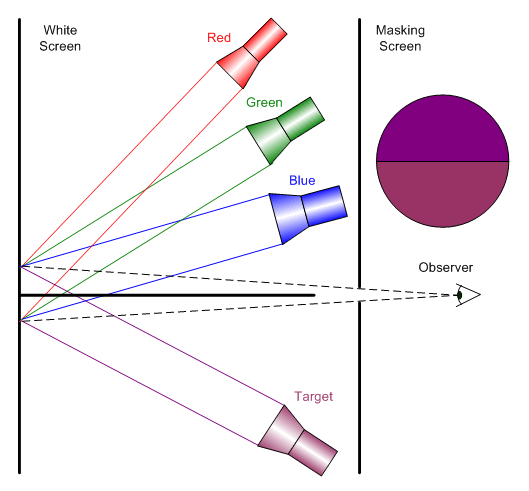
\includegraphics[width=\linewidth]{ColorMatchingExperiment}
\end{minipage}

\subsubsection{Spazio Colore CIE RGB}
\begin{minipage}{0.65\textwidth}
Nel 1931, la CIE standardizzò le funzioni di corrispondenza dei colori RGB ottenute utilizzando i tre primari monocromatici che corrispondono ai colori rosso, verde e blu. Queste funzioni mostrano la quantità di primario necessaria per corrispondere al colore di prova a una determinata lunghezza d'onda. Lo spazio colore CIE RGB è uno tra i tanti spazi colore RGB, distinti da un particolare set di colori primari monocromatici.
\end{minipage}
\begin{minipage}{0.05\textwidth}
\end{minipage}
\begin{minipage}{0.3\textwidth}
    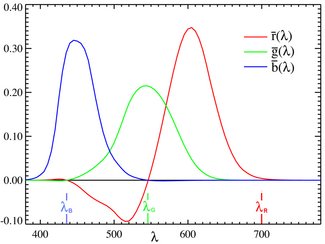
\includegraphics[width=\linewidth]{RGBfunction}
\end{minipage}
\subsubsection{Spazio Colore CIE XYZ}
\begin{minipage}{0.65\textwidth}
Per evitare la presenza di valori negativi nelle funzioni di corrispondenza dei colori CIE RGB, fu sviluppato lo spazio colore CIE XYZ. Lo spazio colore CIE XYZ è collegato allo spazio colore CIE RGB da una trasformazione lineare, progettata in modo che: Y fosse una misura della luminosità o luminanza di un colore; Z fosse quasi uguale alla stimolazione blu; X sia una combinazione lineare delle tre curve di risposta dei coni, scelte per essere non negative.
\end{minipage}
\begin{minipage}{0.05\textwidth}
\end{minipage}
\begin{minipage}{0.3\textwidth}
    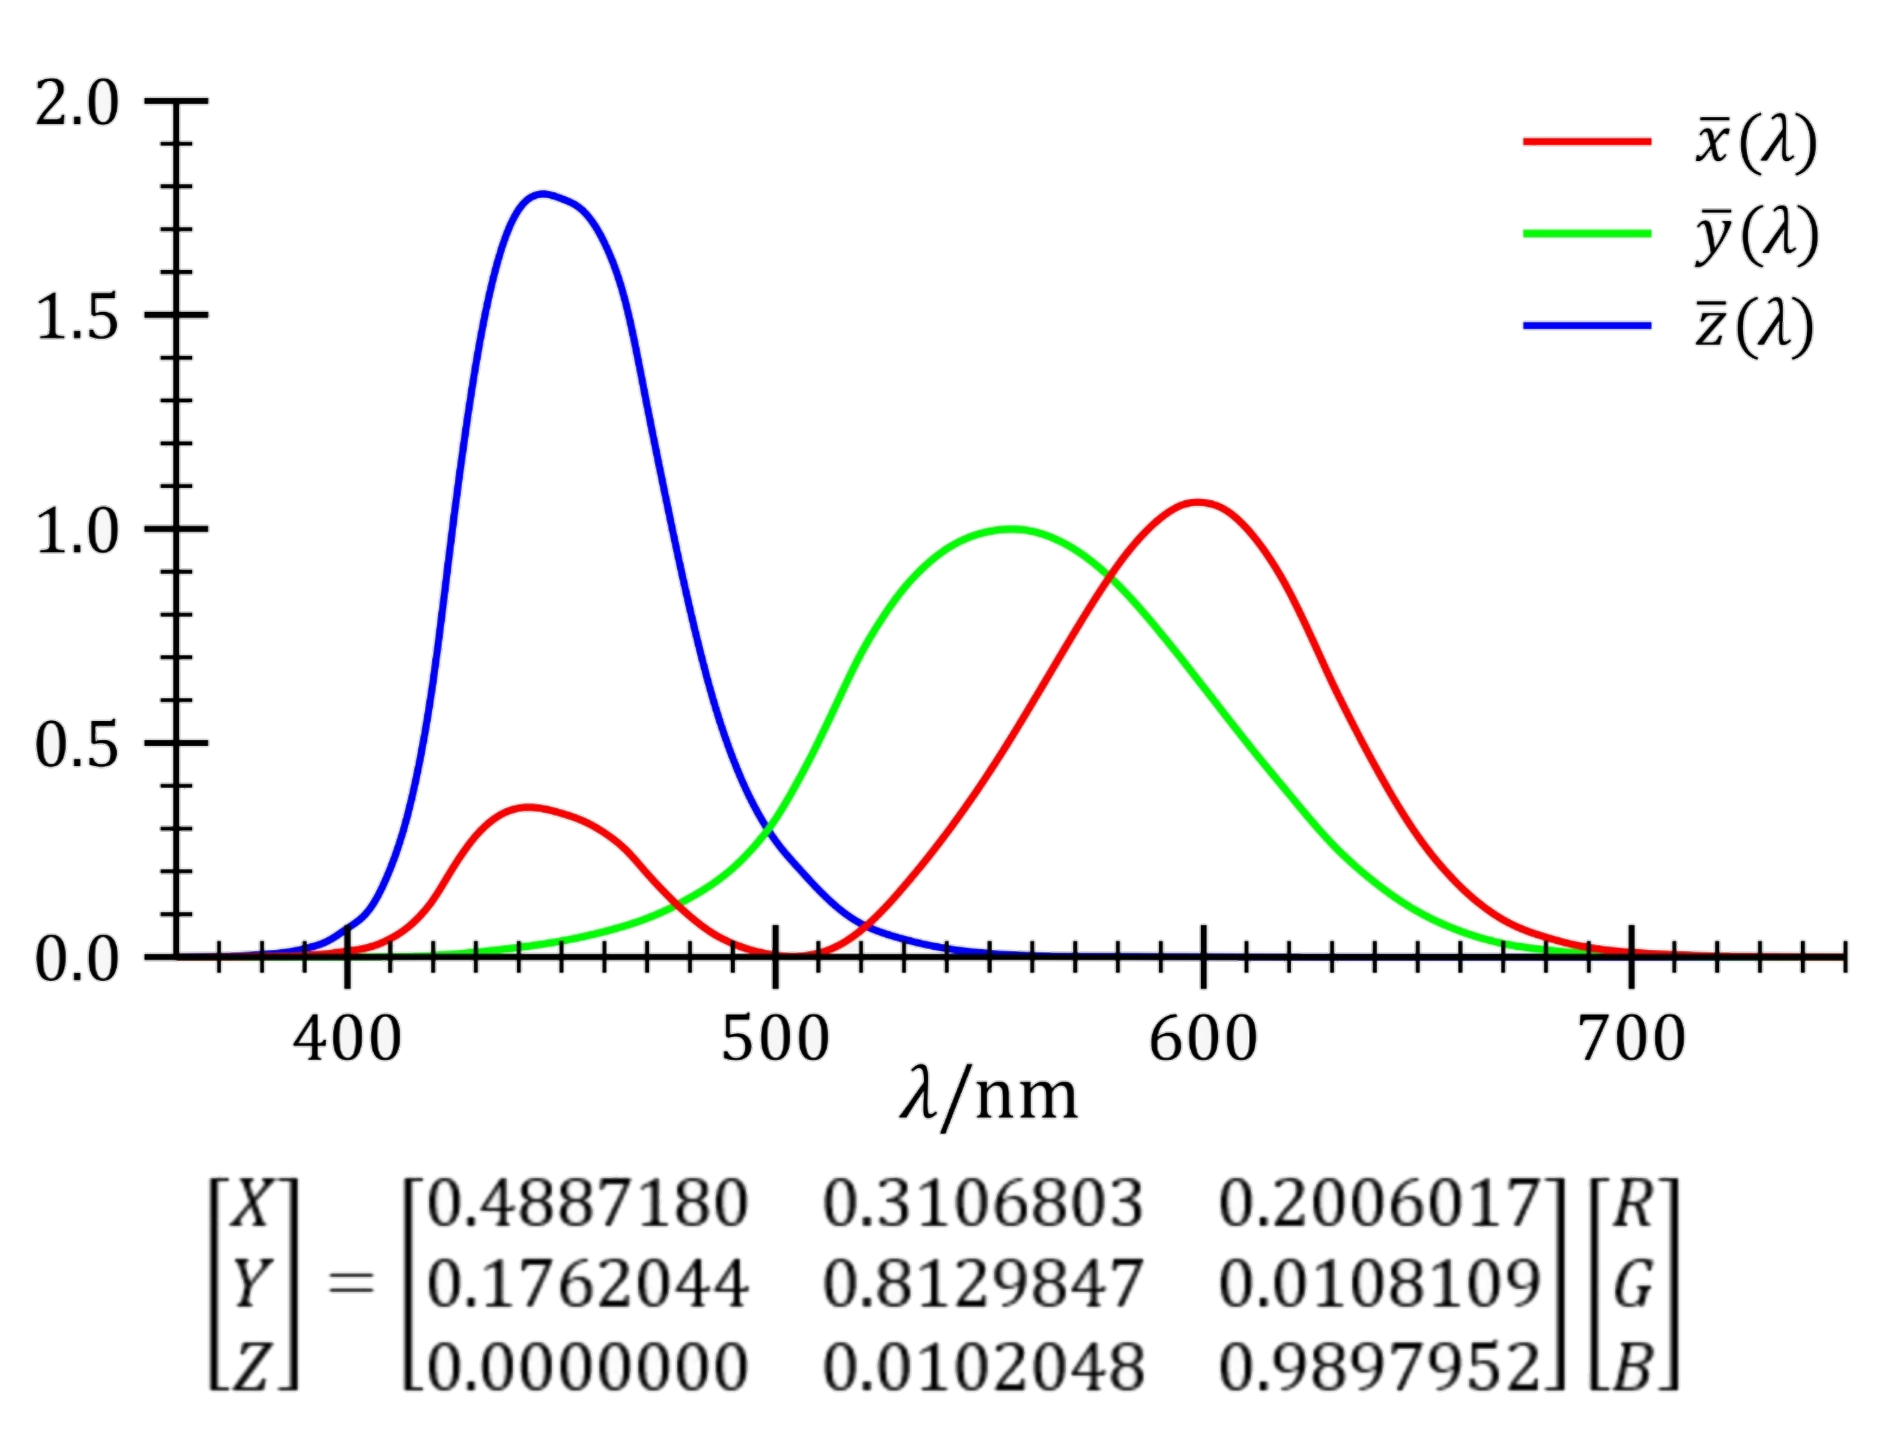
\includegraphics[width=\linewidth]{XYZfunction}
\end{minipage}
\subsubsection{Spazio Colore CIE xyY}
\begin{minipage}{0.65\textwidth}
Definendo Y come luminanza, si ottiene il risultato utile che per un determinato valore di Y, il piano XZ conterrà tutte le cromaticità possibili a quella luminanza. Normalizzando XYZ (cioè dividendo per X+Y+Z), si ottengono valori derivati denominati x, y, z. Essendo x+y+z = 1, la cromaticità di un colore può essere specificata da due parametri x e y, dei tre valori normalizzati, e può essere mappata nel diagramma cromatico CIE.\\
Il diagramma cromatico CIE rappresenta tutti i colori visibili dall'occhio umano con intensità costante pari a 1 (il bianco più luminoso supportato da un display a colori). Il grado di luminanza è espresso dalla coordinata Y di XYZ.
\end{minipage}
\begin{minipage}{0.05\textwidth}
\end{minipage}
\begin{minipage}{0.3\textwidth}
    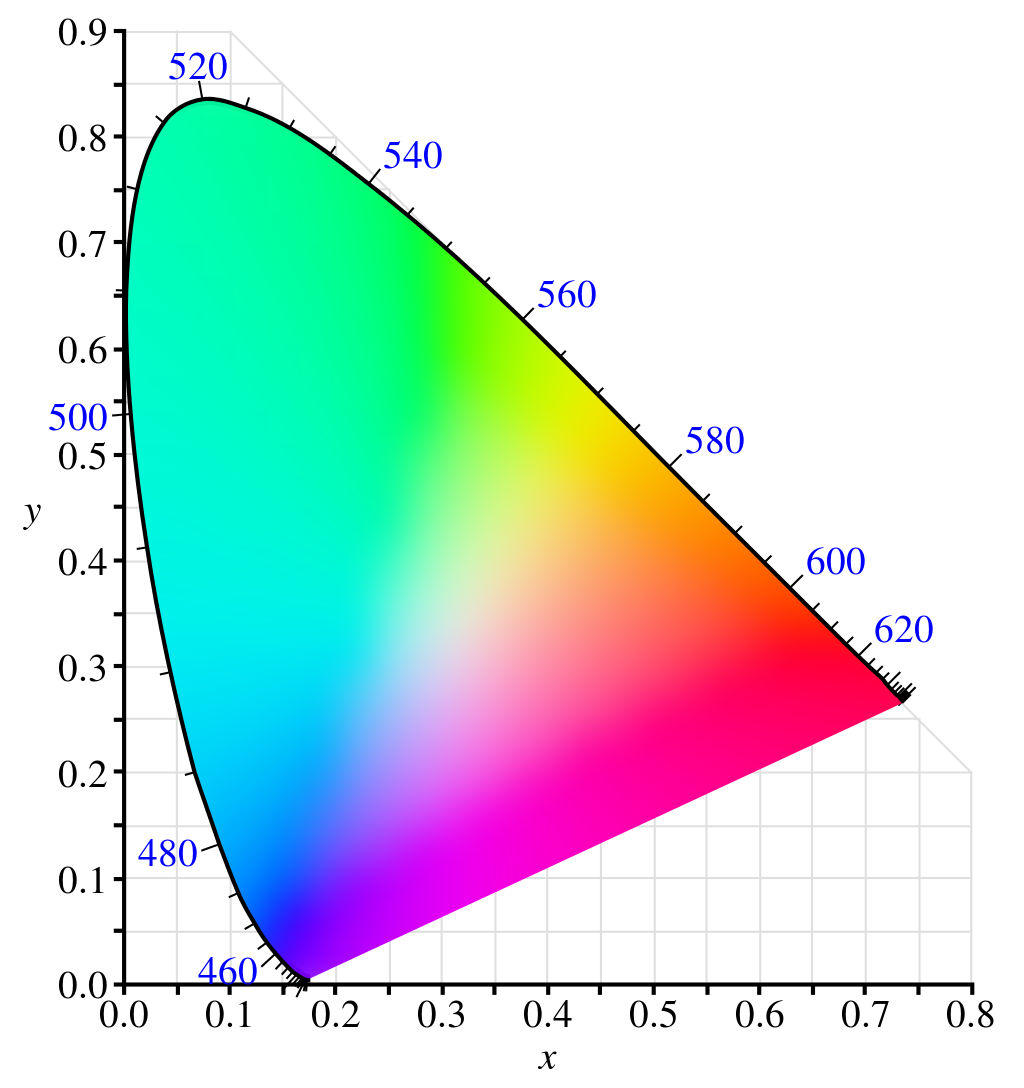
\includegraphics[width=\linewidth]{xyYfunction}
\end{minipage}

\newpage
Esistono anche ulteriori spazi colori, tutti derivati matematicamente dallo spazio colore di riferimento CIE. Ognuno di essi presenta vantaggi e svantaggi particolari, che li rendono utili in applicazioni diverse.

\subsection{Spazio Colore RGB e Derivati}
Lo spazio colore CIE RGB è uno spazio colore additivo, cioè ogni colore è ottenuto dalla somma dei tre primari e può essere rappresentato come un cubo. Lo spazio colore CIE RGB è correlato a XYZ da una trasformazione lineare.\\
Lo spazio colore CIE RGB è uno tra i tanti spazi colore RGB, ognuno dei quali è caratterizzato da un particolare set di colori primari monocromatici (a singola lunghezza d'onda) generati dall'hardware, di fatto dipendendone.\\
Lo spazio colore sRGB (creato in collaborazione da HP e Microsoft nel 1996) è lo spazio colore più usato nella pratica. Utilizza gli stessi primari dello standard ITU-R BT.709, ed è lo standard di riferimento utilizzato per monitor, stampanti e su Internet. Anche schermi LCD, fotocamere digitali, stampanti e scanner seguono tutti lo standard sRGB.\\
\begin{minipage}{0.33\textwidth}
    \centering
    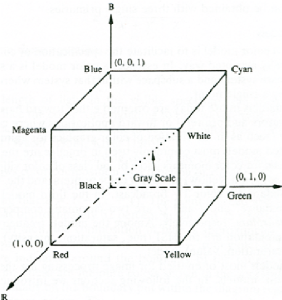
\includegraphics[width=\linewidth]{RGBcube1}
\end{minipage}%
\begin{minipage}{0.34\textwidth}
    \centering
    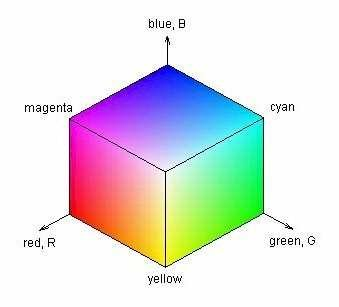
\includegraphics[width=\linewidth]{RGBcube2}
\end{minipage}%
\begin{minipage}{0.33\textwidth}
    \centering
    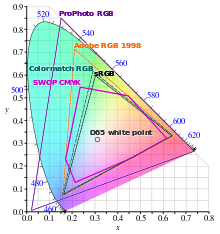
\includegraphics[width=\linewidth]{RGBgamut}
\end{minipage}

\subsection{Rappresentazione Truecolor}
Il numero di uno e zero (bit) utilizzati per creare ogni pixel indica la profondità del colore che è possibile inserire nelle immagini. Il "Truecolor" è un metodo per rappresentare e memorizzare informazioni grafiche dell'immagine, che definisce $256$ $(2^8)$ tonalità di rosso, verde e blu per ogni pixel dell'immagine digitale, risultando in $256^3$ o $16 \, 777 \, 216$ (circa 16,7 milioni) variazioni di colore per ogni pixel.\\
Vengono anche usate profondità di colore di 30, 36 o 48 bit per pixel, anche indicate come 10, 12 o 16 bit per canale RGB, risultando in un miliardo o più di colori.
\begin{figure}[h]
    \centering
    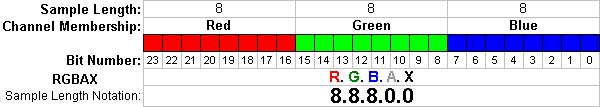
\includegraphics[width=0.8\textwidth]{RGBbit}
\end{figure}

\subsection{Dimensione di File Immagine e Compressione}
La dimensione di un file immagine si calcola moltiplicando l'area dell'immagine per la profondità di bit: \quad $file Size=(pixelDimensions *bitDepth)/8$ (risultato in byte).\\
La compressione si impiega per ridurre le dimensioni dei file delle immagini al fine di facilitare lo stoccaggio, l'elaborazione e la trasmissione. Tutte le tecniche di compressione abbreviano la sequenza di codice binario di un'immagine mediante trasformazioni matematiche basate su algoritmi complessi.

\newpage
\section{Compressione Lossless - Standard di Compressione di Immagini Digitali}

La compressione è il metodo per ottenere una rappresentazione codificata dell'immagine che offre un aspetto simile con un minor numero di bit. La compressione può essere senza perdita (lossless) o con perdita (lossy), che consente un più alto tasso di compressione. La scelta della tecnica di compressione dipende dall'applicazione.

\subsection{Algoritmi di Compressione Lossless}

\subsubsection{Run-Length Coding}
Il run-length coding  è uno schema di codifica a lunghezza fissa, in cui una sequenza di simboli uguali viene codificata con un solo simbolo, preceduto da un simbolo speciale (ad esempio \textdollar) seguito dal numero che specifica quante volte il simbolo appare consecutivamente. Ad esempio:\\
Input string: $aaaaahhbbbbfcccccddddddeeeggggggggggg$ \\
Encoded string: $ \textdollar 5ahh \textdollar 4bf \textdollar 5c \textdollar 6deee \textdollar 11g$\\
In questo caso, se il carattere si ripete meno di 4 volte, è più conveniente scriverlo normalmente invece di codificarlo. Un tempo questo tipo di codifica era usata per le immagini PCX, adesso invece viene usato solo come parti di algoritmi di compressione più complessi (es: JPEG).

\subsubsection{Prefix-free Coding}
Il prefix-free coding è uno schema di codifica in cui ogni simbolo è rappresentato da una codeword, che non è mai il prefisso di qualsiasi altro simbolo. Ogni messaggio codificato in questo modo è quindi univocamente decifrabile, cercandolo in un codebook. \\
\begin{minipage}{0.15\textwidth}
Esempio: \\
A: 00 \\
B: 010\\
C: 011\\
D: 10 \\
E: 11 \\
\end{minipage}
\begin{minipage}{0.45\textwidth}
Messaggio codificato: 1011011000100010\\
Messaggio decodificato: DECABAD
\end{minipage}
\begin{minipage}{0.4\textwidth}
\centering
    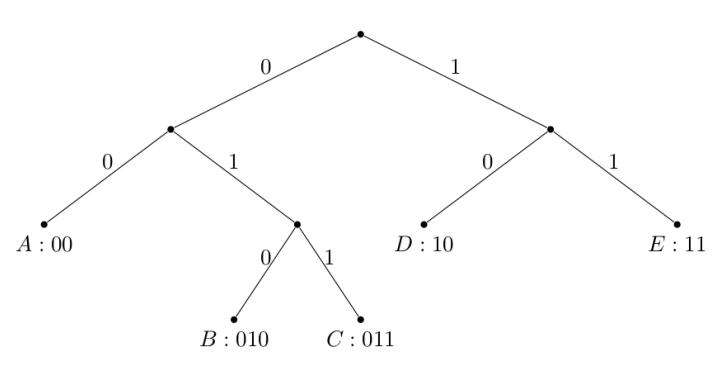
\includegraphics[width=\linewidth]{PrefixFreeTree}
\end{minipage}

\subsubsection{Huffman Coding}
I prefissi usati per i simboli nel prefix-free coding vengono generati tramite l'Huffman coding. Per ogni simbolo viene utilizzato un prefisso che esprime la frequenza con cui esso viene utilizzato, in modo che non sia mai un prefisso di qualsiasi altro simbolo.\\ Può essere generato costruendo un albero binario con nodi contenenti i simboli da codificare e la loro frequenza di occorrenza. L'albero può essere costruito come segue:
\begin{enumerate}
\item selezioniamo i due nodi senza genitori con le frequenze più basse
\item creiamo un nuovo nodo che sia il genitore dei due nodi a frequenza più bassa
\item assegniamo al nuovo nodo una frequenza pari alla somma delle frequenze dei suoi figli
\item ripetiamo dal passo 1 finché non rimane un solo nodo senza genitore
\end{enumerate}
La codifica di ogni simbolo può essere quindi ottenuta tracciando un percorso verso il simbolo a partire dalla radice: 1 viene assegnato per ogni ramo in una direzione e 0 nell'altra. L'esecuzione è abbastanza efficiente, necessitando di $O(n \, logn)$ operazioni per costruirlo. Esempio:\\
Consideriamo una sequenza di 5 con date frequenze e applichiamo i passi\\
\begin{minipage}{0.1\textwidth}
A: 24 \\
B: 12\\
C: 10\\
D: 8 \\
E: 8 \\
\end{minipage}
\begin{minipage}{0.6\textwidth}
1: Combiniamo D e E in DE con frequenza 16\\
2: Combiniamo B e C in BC con frequenza 22\\
3: Combiniamo BC e DE in BCDE con frequenza 38\\
4: Combiniamo A e BCDE in ABCDE con frequenza 62\\
\end{minipage}
\begin{minipage}{0.3\textwidth}
\centering
    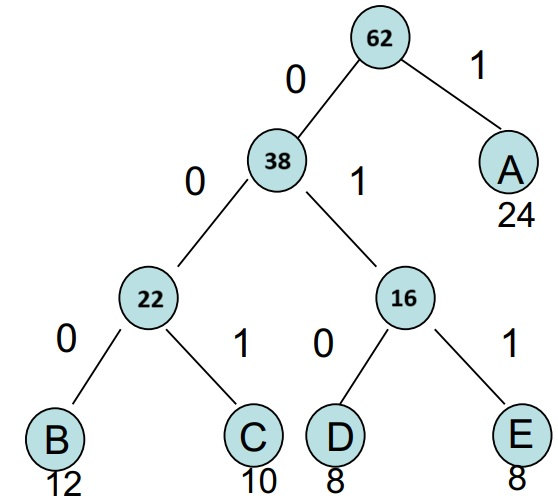
\includegraphics[width=\linewidth]{HuffmanTree}
\end{minipage}
I simboli allora saranno codificati come: \\
A=1 \quad B=000 \quad C=001 \quad D=010 \quad E=011\\
Per codificare il messaggio serviranno quindi 138 bit invece dei 186 originali.\\
Per decodificare i file con codifica Huffman, l'algoritmo di decodifica deve sapere quale codice sia stato usato per codificare i dati: questo può essere fatto tramite una tabella con i simboli e i loro relativi codici, oppure con l'albero. Il metodo più veloce per decodificare consiste nel leggere un bit alla volta e attraversare l'albero fino a raggiungere la foglia contenente il simbolo corrispondente, ricominciando poi dalla radice.\\
Nell'esempio precedente, se la sequenza in ingresso fosse $"1011000010011"$, la sequenza decodificata sarebbe:\quad $A \quad E \quad B \quad D \quad E$.\\
L'algoritmo di Huffman è ottimale quando i simboli dei messaggi non sono correlati fra loro e quando la distribuzione di probabilità in ingresso è nota, ma se così non fosse esistono algoritmi di compressione migliori. \\
Ad esempio la codifica LZW usata nella compressione delle immagini GIF, che si basa sulla frequenza di ripetizione di combinazioni di simboli, può essere più efficiente. 

\subsubsection{LZW Coding}
La compressione LZW, tipicamente utilizzata nei file GIF TIFF e PDF, sostituisce le sequenze formate da 2 o più simboli con un singolo codice, aggiungendo via via le nuove stringhe di simboli ad una tabella. \\
Il codice LZW può essere di lunghezza arbitraria, ma deve necessariamente avere più bit di un singolo simbolo: ad esempio, per i simboli codificati con $8 bit$, è possibile usare codice LZW a $12 bit$; i codici $0/255$ vengono quindi assegnati all'insieme standard dei simboli, mentre i codici $256/4095$ si occuperanno delle stringhe trovate via via che l'algoritmo procede.\\ \\
Esempio - codifica e decodifica LZW: \quad stringa in ingresso "$/WED/WE/WEE/WEB/WET$"\\
\begin{minipage}{0.45\textwidth}
    Supponiamo di assegnare ai singoli simboli i valori $0/255$. \\
    A partire dalla prima coppia di caratteri, viene controllato se la stringa "$/W$" sia presente nella tabella e, dato che non è presente, le viene assegnato il codice $256$.\\
    Dopo la lettura del simbolo "$E$", viene controllata la sequenza "$WE$" e viene aggiunta alla tabella con il codice $257$, stampando poi il codice per "$W$".\\
    Dopo la lettura del simbolo "$D$", viene controllata la sequenza "$ED$" e viene aggiunta alla tabella con il codice $258$, stampando poi il codice per "$E$".
\end{minipage}
\begin{minipage}{0.55\textwidth}
\centering
    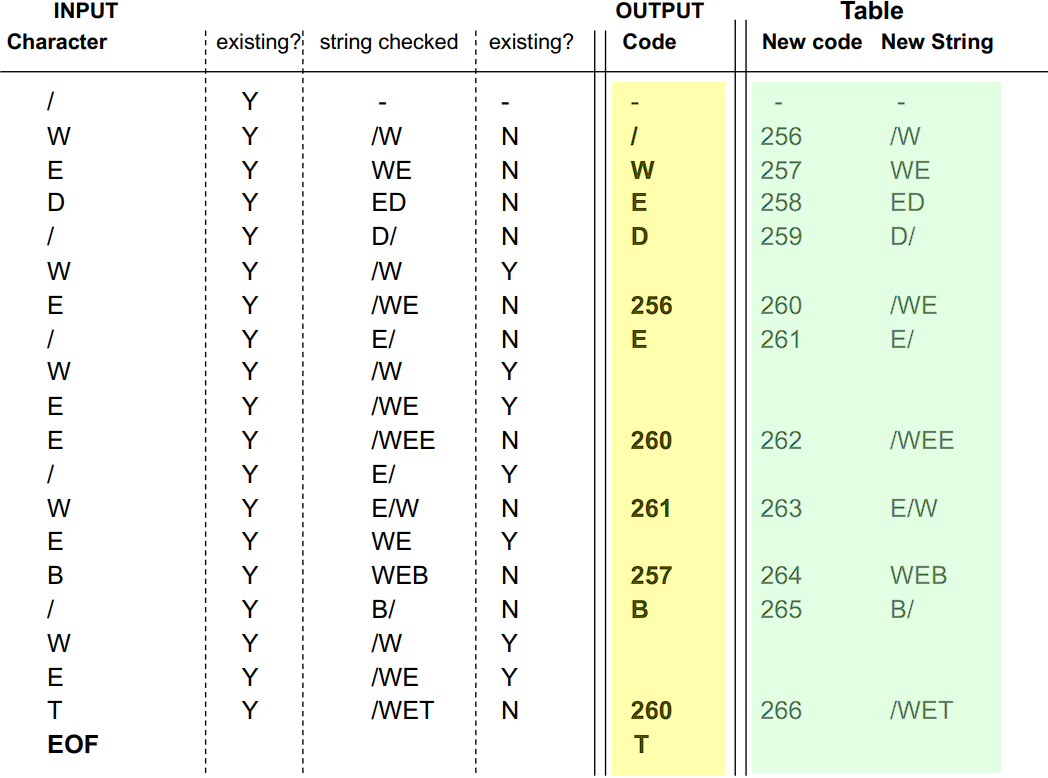
\includegraphics[width=\linewidth]{LZW example.png}
\end{minipage}
Dopo la lettura del simbolo "$/$", viene controllata la sequenza "$D/$" e viene aggiunta alla tabella con il codice $259$, stampando poi il codice per "$D$".
Viene quindi letto il simbolo "$W$" e viene controllata la stringa "$/W$". Dato che questa corrisponde al valore 256 della tabella, viene quindi letto il nuovo carattere "$E$" e si procede a controllare la presenza della stringa "$/WE$". Dato che questa non è presente, viene aggiunta alla tabella con il codice $260$, stampando poi il codice $256$ corrispondente alla sequenza "$/W$".\\
Il processo continua così fino all'esaurimento della stringa e all'emissione di tutti i codici, ottenendo la stringa compressa "$/\,W\,E\,D\,256\,E\,260\,261\,257\,B\,260\,T$". \\
\begin{minipage}{0.45\textwidth}
L'algoritmo di decompressione invece prende la stringa di output appena ottenuta e lo utilizza per ricreare la stringa di input originale. \\Per farlo non ha bisogno di conoscere la tabella usata, in quanto questa può essere ricreata basandosi solamente sull'output generato durante la compressione.
\end{minipage}
\begin{minipage}{0.55\textwidth}
\centering
    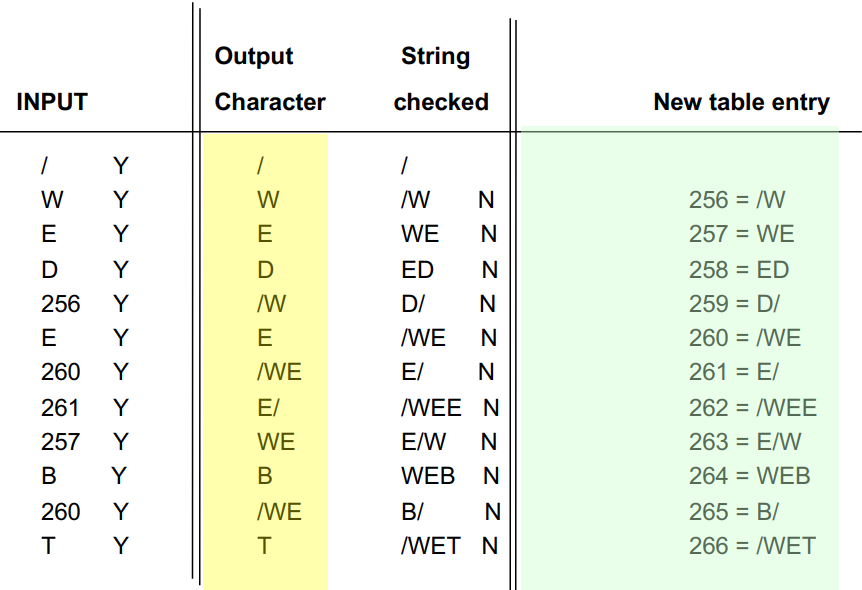
\includegraphics[width=\linewidth]{LZW example 2.png}
\end{minipage}

\subsection{GIF - Graphic Interchange Format}
Il GIF è un formato a $8bit$ per pixel che può usare una palette di massimo $256$ colori scelti nello spazio RGB a $24bit$. Esso utilizza la compressione lossless LZW, presentando quindi immagini con bordi molto nitidi, ed è supportato da tutti i browser.\\
La limitazione a $256$ colori lo rende inadatto alle fotografie o alle immagini con colori continui, mentre è adatto per immagini più semplici come grafici, line-art o loghi.\\
Un tempo molto usato sul web, è stato via via rimpiazzato dal formato PNG, anche se adesso viene utilizzato per GIFs animate, stickers...
\subsubsection{Animazione GIF}
Il formato GIF supporta l'animazione: dopo l'immagine iniziale vengono rappresentate le parti dell'immagine che cambiano dopo ogni frame. Un timer interno conta i frame dell'immagine GIF e la fa ripartire alla fine. È anche possibile avere diverse palette di colori per ogni frame.
\subsubsection{Trasparenza GIF}
I pixel di un'immagine GIF sono normalmente opachi, a meno che uno specifico colore sia designato come trasparente (solo quel colore). Viene usato un processo simile al chroma-key, dove il computer va a cancellare e sostituire i pixel di un colore, tipicamente il verde. 

\subsection{PNG - Portable Network Graphics}
Il PNG è un formato lossless creato per migliorare il formato GIF, superando la sua limitazione a $256$ colori, ed è supportato da tutti i browser.\\
Usando i colori dello spazio RGB a $24bit$ è adatto al trasferimento di immagini su internet. \\
Non supporta però gli image data EXIF (informazioni varie sulle impostazioni della fotocamera, come velocità dell'otturatore, lunghezza focale, esposizione etc...), ed è per questo inadatto per scopi fotografici professionali. \\
\subsubsection{Compressione DEFLATE}
Il formato PNG impiega l'algoritmo di compressione lossless DEFLATE, diviso in due blocchi che utilizzano ognuno una singola modalità di compressione:
\begin{itemize}
\item Compressione LZ77: cerca le stringhe duplicate e le sostituisce con puntatori alla posizione della stessa sequenza trovata prima 
\item Huffman coding: sostituisce i simboli con nuovi simboli ponderati in base alla loro frequenza d'uso
\end{itemize}
Il formato PNG supporta sia immagini in RGB che in scala di grigi. Il numero di canali dipende anche dalla presenza di un canale "alpha", che va a specificare il grado di opacità dei pixel. Le combinazioni di canali possibili sono quindi: 
\begin{itemize}
\item scala di grigi
\item scala di grigi + alpha ($0/1$ indica il livello di trasparenza di ciascun pixel)
\item rosso, verde e blu (RGB / truecolor)
\item rosso, verde, blu e alpha
\end{itemize}

\subsubsection{Compressione LZ77}
individua le sequenze di caratteri che si ripetono, utilizzando una finestra scorrevole di $32K$, ovvero gli ultimi $32768$ caratteri.\\
Quando incontra la stessa sequenza di caratteri già trovata in precedenza le sostituisce con la distanza (ovvero quanto indietro nella finestra si trova la sequenza precedente) e la lunghezza (ovvero il numero di caratteri da controllare se sono identici).\\
Esempio:\\
\begin{minipage}{0.48\textwidth}
Le finestre del dizionario e del buffer scorrono con il cursore. L'output è una tripletta (p,l,c) di valori dove: 
\begin{itemize}
\item p = posizione rispetto al cursore della corrispondenza più lunga che inizia nel dizionario
\item l = lunghezza della corrispondenza più lunga
\item c = il prossimo carattere dopo la corrispondenza più lunga
\end{itemize}
\end{minipage}
\hspace{0.02\textwidth}
\begin{minipage}{0.50\textwidth}
\centering
    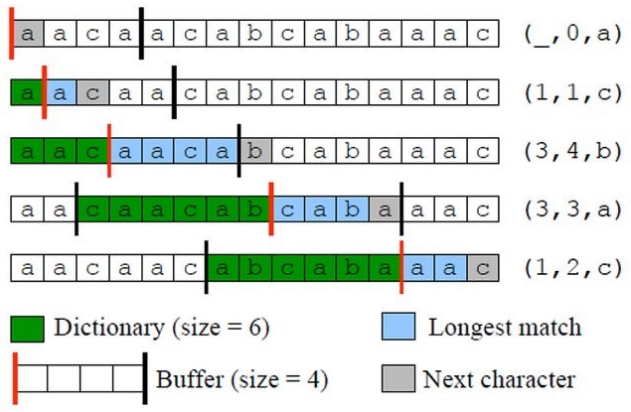
\includegraphics[width=\linewidth]{LZ77 example.png}
\end{minipage}

\newpage

\section{Compressione Lossy - Standard di Compressione di Immagini Digitali}

\subsection{JPEG - Joint Photographic Experts Group}
La compressione lossy JPEG usa il "transform coding", che sacrifica i dettagli dell'immagine per avere una dimensione minore. È il formato più usato per archiviare e trasmettere immagini sul web, perché le immagini JPEG hanno più colori del GIF e hanno dimensione minore rispetto al PNG. Non è però adatto per immagini fatte con linee, testo o icone.\\
Lo standard JPEG specifica sia il codec, che definisce come un'immagine debba essere trasformata in un flusso di bytes, sia il formato JFIF (JPEG File Interchange Format) utilizzato per contenere tale flusso.
La compressione JPEG si basa su due aspetti, ovvero che:
\begin{itemize}
\item la maggior parte dei contenuti utili varia lentamente nelle immagini
\item l'occhio umano è più sensibile alla perdita di dettagli in alta frequenza spaziale rispetto a quelli in bassa frequenza
\end{itemize}
Come risultato quindi si ha che un'immagine, di norma, cambia poco in un'area ridotta e che le componenti a bassa frequenza contengono più informazioni di quelle ad alta frequenza.

\subsubsection{Spazi Colore YCbCr e Y'CbCr}
Per utilizzare lo standard JPEG si passa dallo spazio colore RGB agli spazi YCbCr o Y'CbCr, che consentono una maggiore qualità percettiva dato che assegnano ad un intero canale le informazioni sulla luminosità (canale Y o Y'). La compressione verrà poi applicata singolarmente a ciascun canale.
\begin{itemize}
\item Y (o Y') è la luminanza (o luma), ottenuta come combinazione di R G e B
\item Cb e Cr sono la crominanza del blu e del rosso, ottenuti sottraendo Y (o Y') da B e R 
\end{itemize}

Il luma Y' differisce dalla luminanza Y in quanto è codificato in modo non lineare attraverso una correzione di gamma. La correzione di gamma aiuta a far sì che le immagini digitali appaiano più simili a come le percepiamo con i nostri occhi, ripristinando una relazione lineare tra la luce che colpisce il sensore e la luminosità percepita.\\
Nello standard JFIF è specificata una particolare conversione da RGB a Y'CbCr, da eseguire per ottenere una immagine JPEG con massima compatibilità, definita da:
\begin{align*}
Y' & = 0.299R + 0.587G + 0.114B \\
Cb & = -0.1687R - 0.3313G + 0.5B + 128 \\
Cr & = 0.5R - 0.4287G - 0.0813B + 128 \\
\end{align*}



\subsubsection{Chroma Subsampling}
Possono essere usati 4 diversi livelli di sottocampionamento: 
\begin{itemize}
\item 4:4:4 = la risoluzione della crominanza è preservata allo stesso modo della luminanza
\item 4:2:2 = nella crominanza si perde metà della risoluzione orizzontale, lasciando quella verticale uguale alla luminanza
\item 4:1:1 = viene preservato solo $\frac{1}{4}$ della crominanza orizzontale rispetto alla luminanza
\item 4:2:0 = si perde metà dell'informazione sia orizzontale che verticale della crominanza
\end{itemize}

\subsubsection{Fasi Principali dell'Algoritmo}
Inizialmente l'immagine viene divisa in blocchi piccoli da $8*8$ pixel, aggiungendo righe e colonne clone dell'ultima in caso le dimensioni non siano multiple di $8$, per rimuovere le componenti ad alta frequenza. L'algoritmo viene eseguito su ogni sottoimmagine $8*8$, i passi sono: \\

\begin{minipage}{0.4\textwidth}
\begin{enumerate}
\item DCT - trasformata discreta del coseno
\item Quantizzazione
\item Scansione a zig-zag
\item Codifica dell'entropia
\end{enumerate}
Quest'ultima è a sua volta divisa in:
\begin{enumerate}
\item Codifica dei coefficienti (DPCM su componenti DC, RLE su componenti AC)
\item Codifica Huffman
\end{enumerate}
\end{minipage}
\hspace{0.05\textwidth}
\begin{minipage}{0.55\textwidth}
\centering
    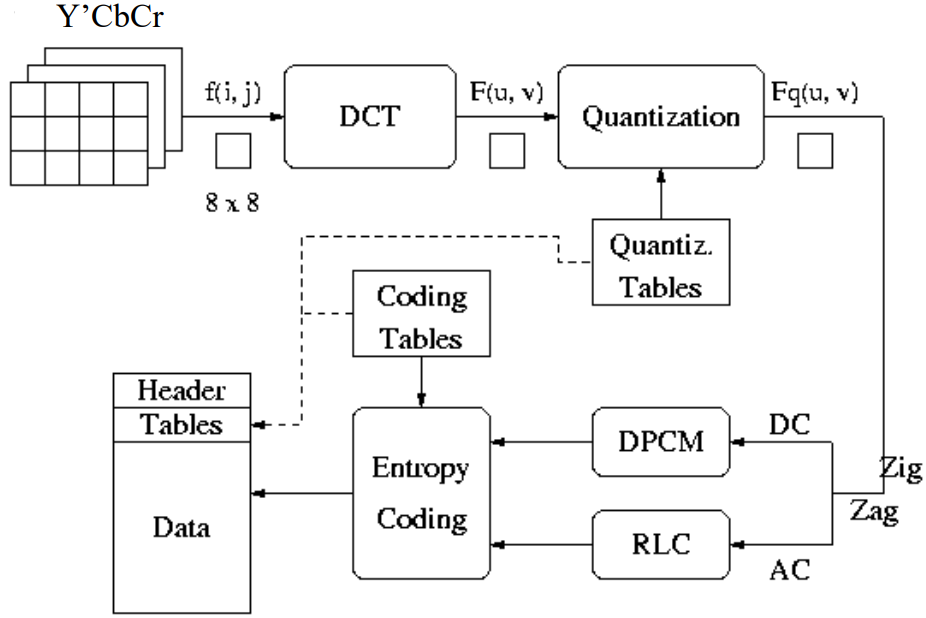
\includegraphics[width=\linewidth]{JPEG chain.png}
\end{minipage}

\subsubsection{DCT - Trasformata Discreta del Coseno}
Tramite la DCT passiamo dal dominio spaziale a quello della frequenza, secondo la formula: 
$$
F(u,v)=\frac{\Delta(u) \Delta(v)}{4} \sum_{i=0}^7 \sum_{j=0}^7 \cos \frac{(2i+1)u \pi}{16} \cos \frac{(2j+1)v \pi}{16} f(i,j)\, , \quad  \Delta(\epsilon)=
\begin{cases}
\frac{1}{\sqrt{2}}, & \text{se } \epsilon = 0 \\
1, & \text{altrimenti}
\end{cases}
$$

\begin{minipage}{0.65\textwidth}
Nella formula $f(i,j)$ rappresenta i valori presenti nelle posizioni $(i,j)$ del blocco $8*8$ dell'immagine originale, mentre $F(u,v)$ sono i valori dei coefficienti DCT nelle posizioni $(u,v)$ della matrice $8*8$ dei coefficienti trasformati.

Così facendo andiamo a mettere le componenti in più bassa frequenza (valori molto alti) nelle celle in alto a sinistra, mentre quelle in alta frequenza (valori molto piccoli) in basso a destra. Spostandosi lungo le righe aumentiamo la frequenza verticale, spostandosi lungo le colonne quella orizzontale.
\end{minipage}
\hspace{0.05\textwidth}
\begin{minipage}{0.3\textwidth}
\centering
    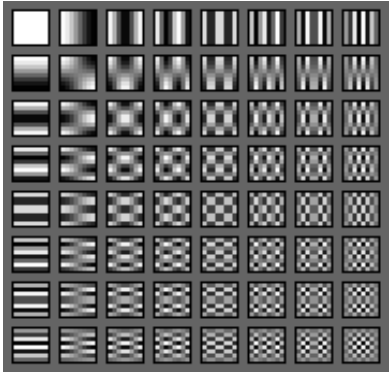
\includegraphics[width=\linewidth]{DCT visualization.png}
\end{minipage}
\\\\
Esempio:
\begin{figure}[h]
\centering
\begin{minipage}[b]{0.5\textwidth}
\centering
    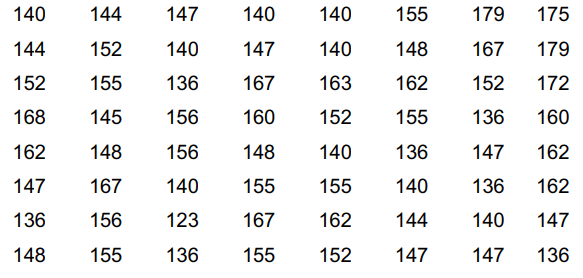
\includegraphics[width=\linewidth]{DCT example 1.png}
    \caption{Valori in ingresso}
\end{minipage}%
\begin{minipage}[b]{0.5\textwidth}
\centering
    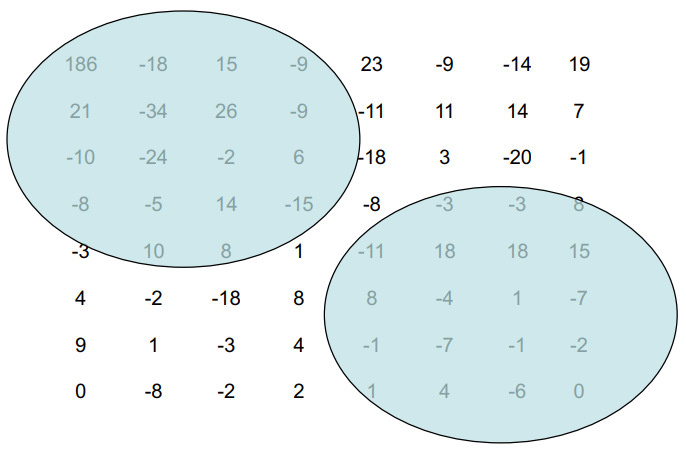
\includegraphics[width=\linewidth]{DCT example 2.png}
    \caption{Valori DCT di uscita}
\end{minipage}
\end{figure}

\subsubsection{Quantizzazione}
La quantizzazione viene usata per ridurre notevolmente il numero di bit per campione, ed è anche la fonte principale di perdita di informazione.
Per farlo va a dividere ed arrotondare all'intero più vicino i valori della matrice ottenuta con la DCT, secondo la formula: 
$$F'[u,v]=round(F[u,v]/ q[u,v])$$
dove $q[u,v]$ è detta matrice di quantizzazione, della quale esistono vari tipi:
\begin{itemize}
\item Quantizzazione uniforme: ogni coefficiente $F[u,v]$ viene diviso per la stessa costante $N$
\item Quantizzazione non uniforme: tiene conto che l'occhio umano è più sensibile alle basse frequenze rispetto a quelle alte, ed è più sensibile alla luminanza rispetto che al colore
\end{itemize}
\begin{figure} [h]
\centering
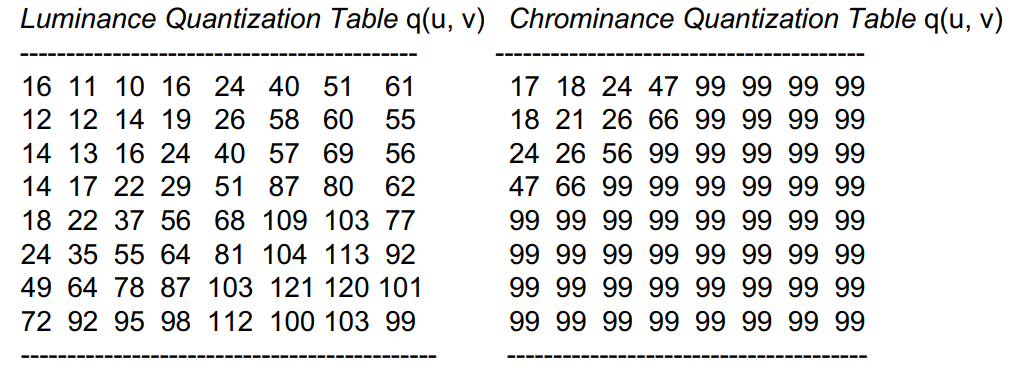
\includegraphics[width=0.7\textwidth]{Quantization tables}
\end{figure}

\subsubsection{Scansione a Zig-Zag}
\begin{minipage}{0.7\textwidth}
Come risultato della quantizzazione avremo una matrice $8*8$ con molti valori uguali a 0, e i valori diversi da 0 saranno concentrati in alto a sinistra. Trasformiamo quindi la matrice in un vettore di $64$ elementi andando "a zig-zag", in modo da raggruppare i coefficienti delle basse frequenze (diversi da 0) in cima al vettore.
\end{minipage}
\hspace{0.1\textwidth}
\begin{minipage}{0.2\textwidth}
\centering
    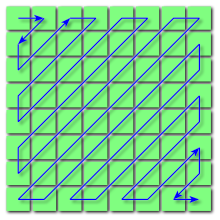
\includegraphics[width=\linewidth]{ZigZag scan.png}
\end{minipage}
\\
\subsubsection{Codifica dei Coefficienti}
La codifica dei coefficienti si divide in: 
\begin{itemize}
\item DPCM (differential pulse code modulation) sulla componente DC: la componente DC è ampia e variegata, ma comunque con valore simile ai blocchi vicini; l'algoritmo JPEG quindi codifica la differenza tra il blocco $8*8$ precedente e quello corrente
\item RLE (run length encoding) sulle componenti AC: molti dei coefficienti AC sono pari a 0, per questo è conveniente usare il RLE che conta il numero di 0 consecutivi, terminando poi il blocco con $(0,0)$
\end{itemize}
Per il componente DC avremo quindi la coppia $(SIZE)(AMPLITUDE)$ dove SIZE è il numero di bit necessari a rappresentare il valore DC e AMPLITUDE è il valore della differenza DC. Per le componenti AC invece avremo la rappresentazione $(RUNLENGTH,SIZE)(AMPLITUDE)$ dove RUNLENGTH è il numero di 0 consecutivi, SIZE è il numero di bit necessari a rappresentare il valore e AMPLITUDE è il valore dei coefficienti diversi da 0.
\newpage
Esempio: 
\begin{figure} [h]
\centering
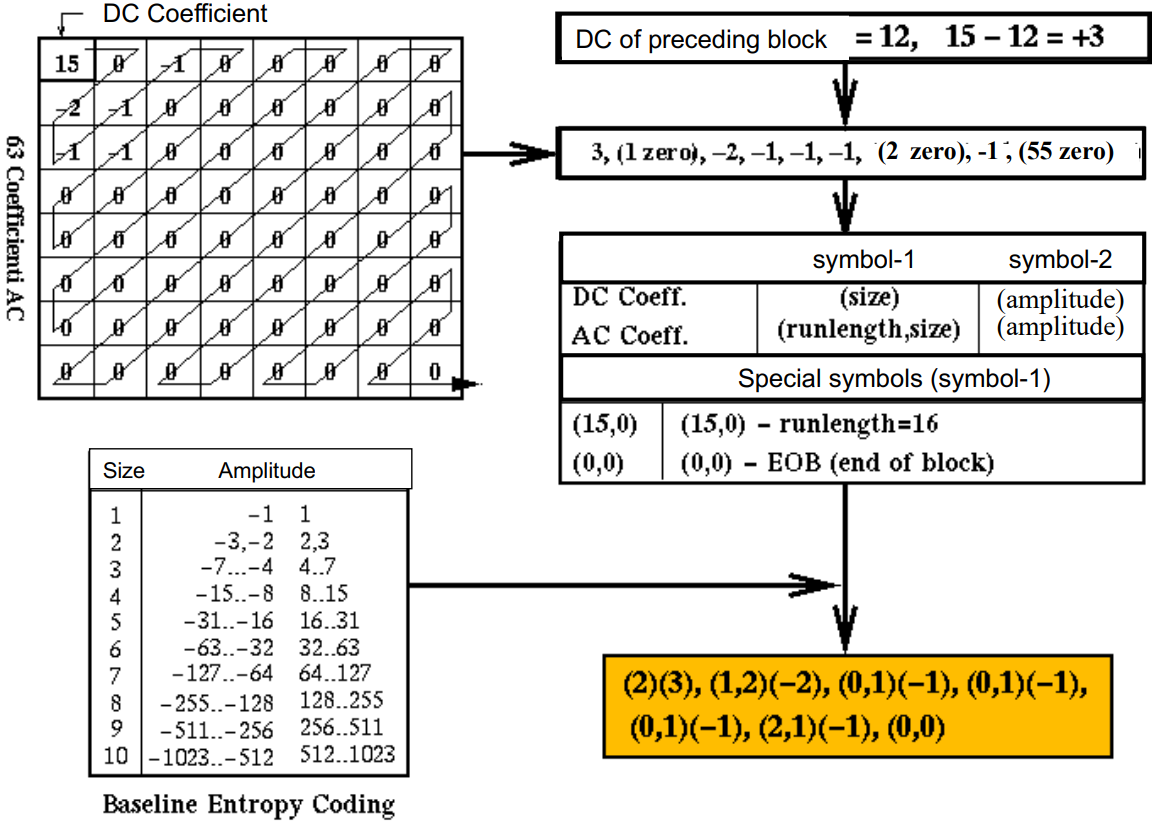
\includegraphics[width=0.6\textwidth]{Coefficient encoding}
\end{figure}

\subsubsection{Codifica Huffman}
Dopo aver codificato ogni blocco avremo quindi una serie di simboli: 
\begin{itemize}
\item Simbolo 1: $(SIZE)$ oppure $(RLE,SIZE)$
\item Simbolo 2: $(AMPLITUDE)$
\end{itemize}
Questi simboli vengono codificati ulteriormente usando Huffman, dove i simboli più frequenti sono codificati con codice più breve. Le tabelle di Huffman possono essere di default oppure custom inviandole nell'header dell'immagine.

In conclusione quindi un'immagine JPEG verrà codificata come segue: 
\begin{figure} [h]
\centering
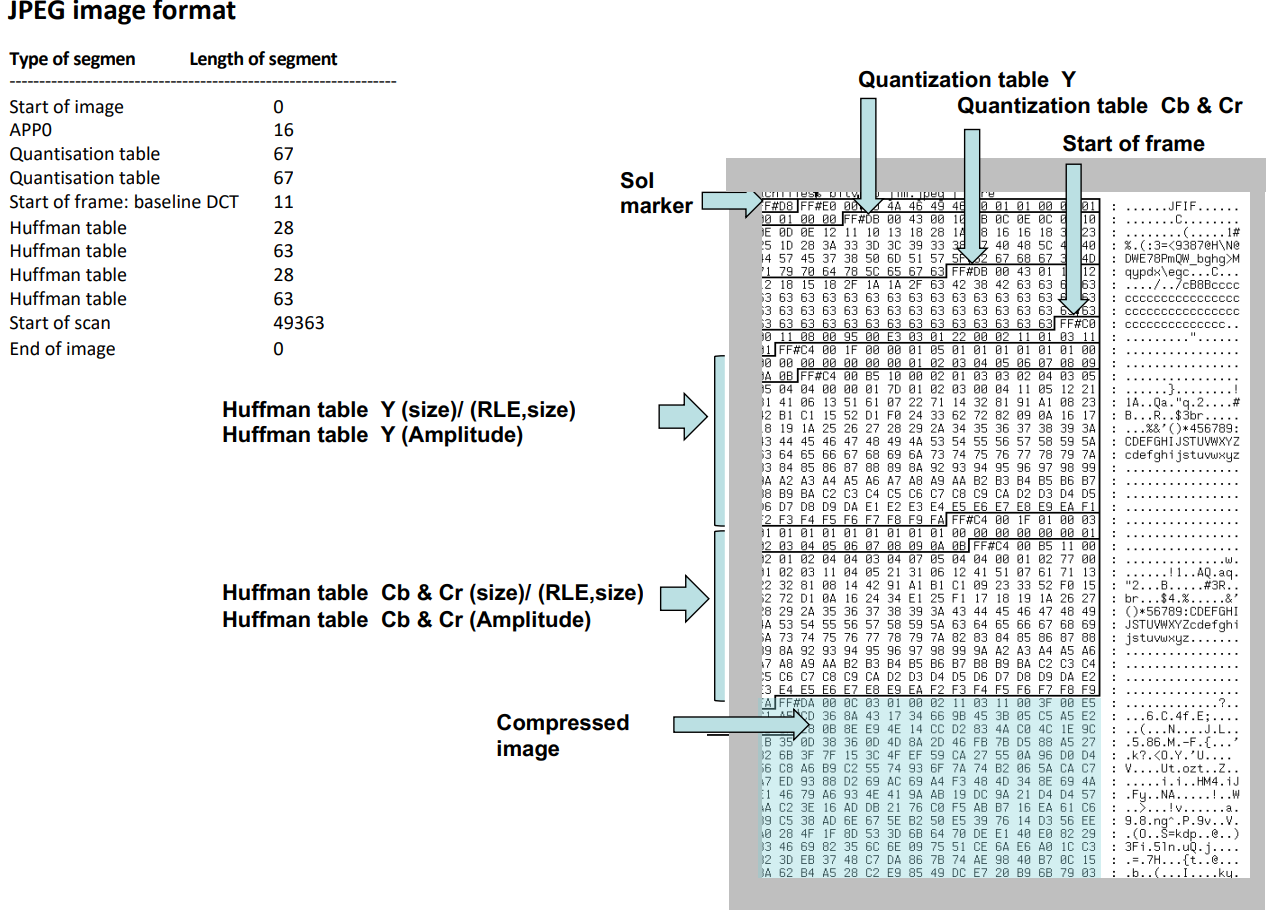
\includegraphics[width=0.9\textwidth]{JPEG format}
\end{figure}

\newpage
\subsection{Standard a Confronto - GIF, PNG, JPEG}
I formati GIF e PNG usano entrambi una compressione senza perdita, ottenendo livelli medi di compressione: 
\begin{itemize}
\item GIF funziona meglio su immagini con pochi colori o immagini dove un colore è dominante; non ha perdita purché l'immagine originale abbia meno di 256 colori; hanno inoltre il vantaggio di poter usare la trasparenza e l'animazione.
\item PNG è l'alternativa senza perdita per quando si hanno più colori
\end{itemize}
Il formato JPEG è con perdita, ma ottiene alti livelli di compressione. La compressione funziona bene per immagini a tonalità continua, ovvero dove la variazione tra pixel adiacenti è piccola. A causa della notevole perdità di qualità, è bene usare JPEG quando la dimensione dei file è importante, ad esempio nelle pagine web.\\
JPEG è quindi lo standard per la fotografia digitale, dove si riescono ad ottenere file molto più piccoli dei corrispettivi PNG perdendo relativamente pochi dettagli. PNG è invece la scelta migliore se abbiamo immagini contenenti testo, line art o transizioni nette.\\
Alcune regole generali sono: 
\begin{itemize}
\item GIF: immagini in bianco e nero, testo su sfondo a tinta unita, immagini con trasparenza o animate, line-art o cartoon-art fatta a computer, icone, pulsanti, immagini con un colore prevalente ($>80\%$)
\item JPEG: fotografie scannerizzare a $16/24$ bit, immagini fatte a computer con toni continui, immagini e fotografie scannerizzate, immagini grandi con molti dettagli 
\end{itemize}

\newpage
\section{Video Digitali}
Un video è una sequenza di frame (immagini), di norma a $24/30$ fps, in modo da apparire all'occhio umano come un flusso continuo di informazione. Il video analogico è un segnale analogico che contiene luminanza e crominanza, ma non è più in uso a favore del video digitale, ovvero una sequenza rapida di immagini in successione. Come per le immagini, ne esistono formati compressi come il H.264 e il H.265. \\
I vantaggi del video digitale sono: 
\begin{itemize}
\item può essere copiato senza perdita di qualità
\item può essere manipolato o editato su computer
\item registrare video digitale è molto economico
\end{itemize} 
Per questi motivi si è via via affermato in ambito televisivo, nell'industria cinematografica e sul web, via via aumentando di qualità e introducendo compressioni più efficienti. Aspetti fondamentali del video digitale sono: formati di cattura, spazi colore, codifica, risoluzione, aspect ratio (proporzioni), bitrate, sampling (campionamento) e gli standard di compressione.

\subsection{Formati di Cattura}
Esistono due diversi formati di cattura per i video digitali: interlacciato e progressivo
\begin{itemize}
\item Interlacciato: le videocamere interlacciate catturano le immagini a set alternati di righe, prima vengono scansionate le righe dispari e successivamente quelle pari. Un set di righe dispari o pari viene chiamato field e una coppia di field consecutivi viene chiamata frame.
\item Progressivo: le videocamere progressive scannerizzano ogni singolo frame in modo distinto, catturando tutte le linee dell'immagine nello stesso momento.
\end{itemize}

\subsubsection{Video Interlacciati}
I video interlacciati erano stati introdotti inizialmente quando non era possibile trasmettere una grande quantità di dati, in modo che il video risultasse più fluido all'occhio umano. Questo però ha introdotto alcune inefficienze, soprattutto in video contenenti oggetti che si muovono velocemente o contenenti dettagli orizzontali, portando ad avere degli interlacing effects. 

\begin{figure} [h]
\centering
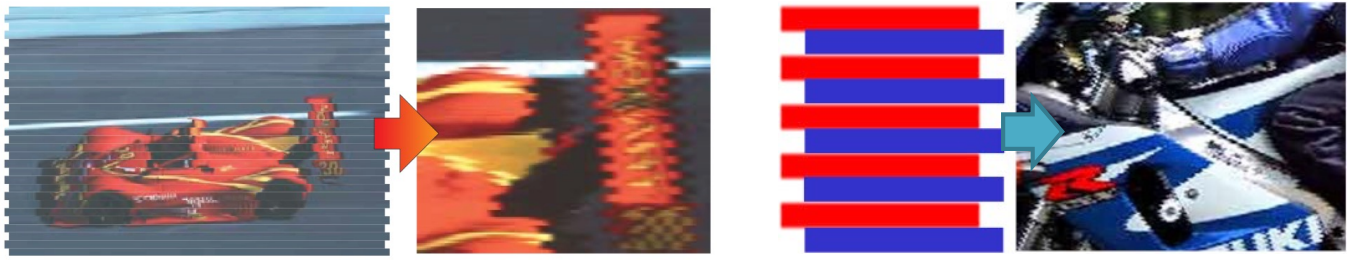
\includegraphics[width=\textwidth]{Interlacing effects}
\end{figure}
Oggi il video interlacciato è sempre meno in uso: rimane supportato da alcune videocamere digitali e, per essere riprodotto, ha bisogno di alcuni processi di deinterlacciamento. \\
Nel caso di un video interlacciato, la sua risoluzione può essere identificata da una i posta accanto al numero, come ad esempio: $1080i$.

\subsection{Spazi Colore}
I video vengono riprodotti in RGB sui monitor, ma vengono trasmessi e conservati usando gli spazi colore YCbCr o Y'CbCr in modo da distinguere le informazioni di luminanza e crominanza. 

\subsection{Codifica}
La luminanza e la crominanza delle immagini che compongono un video possono essere trasportate combinate in un unico canale (composite encoding) oppure tramite canali separati (component encoding). 
\begin{itemize}
\item I video analogici possono usare sia il composite che il component encoding
\item I video digitali usano esclusivamente il component color encoding
\end{itemize}

\subsection{Risoluzione}
Esistono varie risoluzioni per i video digitali, le più note sono: 
\begin{itemize}
\item SD (Standard Definition) 675p: $720*576$ pixel se in $4:3$, $1024:576$ pixel se in $16:9$
\item HD (High Definition) 720p: $1280*720$ pixel
\item HD 1080i/1080p (Full HD): $1920*1080$ pixel in modo interlacciato o progressivo
\item ULTRA HD 4K: $3840*2160$ pixel per la tv, $4096*2160$ per il cinema
\item ULTRA HD 8K: $7680*4320$ pixel per la tv, $8192*4320$ per il cinema
\end{itemize}

\subsection{Aspect Ratio - Proporzioni}
L'aspect ratio di un'immagine descrive le proporzioni tra la sua larghezza ed altezza. Gli standard principali sono 2: 
\begin{itemize}
\item 4:3 (1.33:1): usato dalla creazione dei video, è usato nella standard television
\item 16:9: più moderno, è lo standard per la HDTV 
\end{itemize}
Ci sono anche altri formati, come quello quadrato o verticale, via via più usati perché più adatti per i dispositivi mobili.

\subsection{Bitrate}
Il bitrate è l'equivalente nei video della larghezza di banda: misura la quantità di bit inviati per unità di tempo (bits per second), più è alto e più informazioni vengono inviate:\\

\begin{minipage}{0.3\textwidth}
\begin{itemize}
\item 16 Kbit/s
\item 128-364 Kbit/s
\item 1.25 Mbit/s
\item 5 Mbit/s
\item 8-16 Mbit/s
\item 29.4 Mbit/s
\item 50 Mbit/s\\
\end{itemize}
\end{minipage}
\begin{minipage}{0.7\textwidth}
\begin{itemize}[label={}]
\item per i videotelefoni
\item per le videoconferenze con compressione video
\item per i CD con compressione MPEG1
\item per i DVD con compressione MPEG2
\item per la HDTV con compressione MPEG4
\item per i video in FULL HD
\item per i video in 4K ULTRA HD\\
\end{itemize}
\end{minipage}

Il bitrate può essere costante oppure variabile: 
\begin{itemize}
\item Constant bitrate (BCR): mantiene lo stesso bitrate per tutto il video, ma può produrre video di qualità non uniforme dovendo comprimere di più le parti di video più complesse
\item Variable bitrate (VBR): per massimizzare la qualità video e minimizzare il bitrate, vengono usati più bit nelle scene più complesse e meno in quelle meno complesse, in modo da ottenere una qualità visiva uniforme
\end{itemize}

\section{Compressione di Video Digitali}
È sempre necessaria una certa quantità di compressione nei file: più alta è la risoluzione e più basso è il bitrate, più compressione sarà necessaria e più dati verranno persi.\\ 
Gli algoritmi di compressione tentano quindi di ridurre la quantità di informazioni mantenendo la qualità video, e sono in generale di tipo lossy.\\
Un codec (o coder/decoder) è uno strumento di codifica che processa il video e lo memorizza in un flusso di byte. I codec usano algoritmi per diminuire la dimensione dei file, decomprimendoli poi quando necessario:
\begin{itemize}
\item Gli algoritmi possono essere sia simmetrici che asimmetrici in termini di tempo e complessità di (de)compressione; tipicamente sono molto asimmetrici.
\item La compressione è sia spaziale che temporale, cioè rimuove dati ridondanti sia spazialmente (tipo JPEG) che temporalmente.
\end{itemize}
Per la trasmissione di video in diretta i sistemi di codec video sono generalmente connessi in cascata, cercando di limitare il più possibile la degradazione della qualità. 
\begin{figure} [h]
\centering
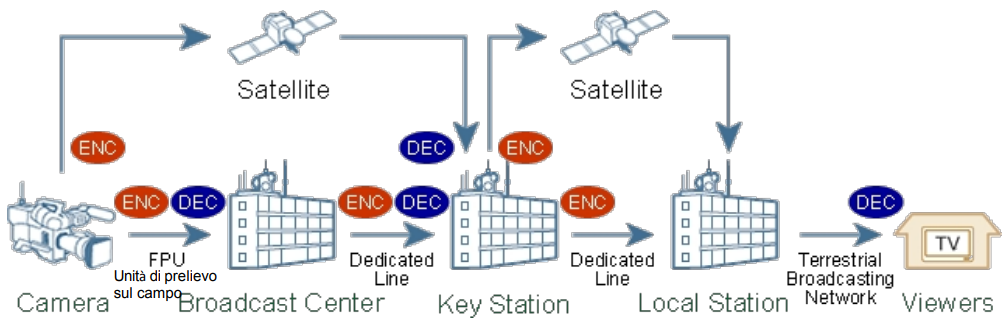
\includegraphics[width=0.8\textwidth]{Compression cascading}
\end{figure}

\subsection{Sampling}
Il sampling (campionamento) è il meccanismo più semplice per la compressione video; viene applicato alla luminanza e alla crominanza di ogni frame video.\\
Viene espresso con tre valori:
\begin{itemize}
\item x = numero relativo di campioni della luminanza (Y), normalmente 4
\item y = numero di campioni della crominanza (CbCr) per le linee dispari
\item z = numero di campioni della crominanza (CbCr) per le linee pari
\end{itemize}

\begin{minipage}{0.3\textwidth}
\centering
    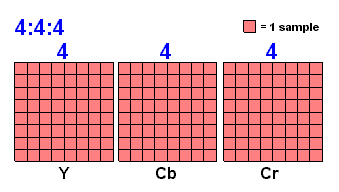
\includegraphics[width=\linewidth]{Sampling 444.png}
\end{minipage}%
\hspace{0.05\textwidth}%
\begin{minipage}{0.3\textwidth}
\centering
    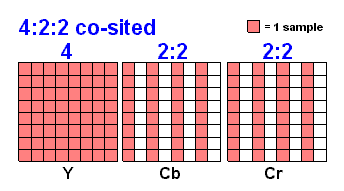
\includegraphics[width=\linewidth]{Sampling 422.png}
\end{minipage}%
\hspace{0.05\textwidth}%
\begin{minipage}{0.3\textwidth}
\centering
    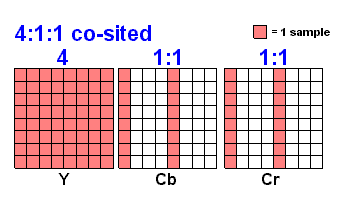
\includegraphics[width=\linewidth]{Sampling 411.png}
\end{minipage}

\hspace{0.15\textwidth}%
\begin{minipage}{0.3\textwidth}
\centering
    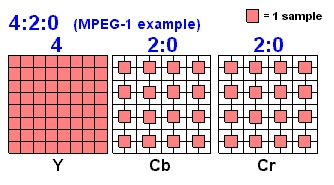
\includegraphics[width=\linewidth]{Sampling 420 1.png}
\end{minipage}%
\hspace{0.05\textwidth}%
\begin{minipage}{0.3\textwidth}
\centering
    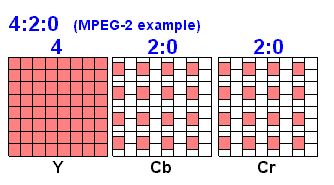
\includegraphics[width=\linewidth]{Sampling 420 2.png}
\end{minipage}%
\hspace{0.15\textwidth}%

\subsection{Standard di Compressione}
Considerare un video come una semplice sequenza di frame, applicando le compressioni studiate per le immagini, è molto riduttivo: in questo modo non andremmo a considerare il fatto che, nel tempo, alcune parti di un video rimangono uguali o simili. Per questo motivo sono stati via via introdotti nuovi standard di compressione appositi per i video.

\subsubsection{Compressione MPEG}
I metodi di compressione MPEG mirano a ridurre la ridondanza nelle sequenze video. MPEG definisce il protocollo di flusso dei bit tra l'encoder e il decoder; l'encoder stesso e il decoder non sono specificati, ma sono lasciati da fare agli sviluppatori. \\
Nel corso degli anni sono stati create diverse versioni del protocollo MPEG:
\begin{itemize}
\item MPEG-1 H.261: usato per VHS, video-CD e audio MP3
\item MPEG-2 H.262: usato per broadcasting, DTTV, TV satellitare e DVD
\item MPEG-4 H.242: il più usato oggi per TV, mobile, internet, blu-ray etc...
\item MPEG-H H.265: ad alta efficienza, usato attualmente per videosorveglianza
\end{itemize}

\subsubsection{Container Video}
I video sono accessibili agli utenti tramite dei container (contenitori), che hanno lo scopo di contenere tutti i file audio, video e codec compressi in un unico pacchetto. I container spesso contengono anche informazioni aggiuntive come informazioni sui capitoli dei film, metadati, sottotitoli o diverse tracce audio. I più popolari sono: 
\begin{itemize}
\item MKV (open source)
\item MP4 
\item AVI, WMV, ASF (Microsoft)
\item MOV (Apple)
\item XAVC, XAVC-S (Sony)
\item FLV, SWF (Flash Video)
\end{itemize}

\subsection{MPEG-1 H.261}
Originalmente sviluppato per supportare la qualità video VHS (videocassette) a circa 1.5Mbps, supportando solo video progressivi, si basa su due principi fondamentali: 
\begin{itemize}
\item un video è una semplice successione di immagini ferme
\item la differenza tra due immagini adiacenti è generalmente piccola
\end{itemize} 
Basandosi su questi concetti fondamentali, le caratteristiche principali dell'MPEG1 sono: 
\begin{itemize}
\item intra-frame coding: compressione sulla transformazione del dominio, simile alla DCT, quantizzazione e RLE del JPEG, 
\item inter-frame coding: blocchi simili di pixel in frame adiacenti vengono rimpiazzati da dei puntatori (motion vector) riferiti a quelli di un frame ancora
\end{itemize}

\subsubsection{Struttura del Bit-Stream}
\begin{minipage}{0.6\textwidth}
\begin{itemize}
\item Sequence layer: dimensioni dell'immagine, aspect-ratio, dimensione minima del buffer, matrici DCT
\item GOP layer: unità per accesso random
\item Picture layer: unità di codifica primaria
\item Slice layer: unità di sincronizzazione
\item Macrobook layer: unità di compensazione del moto
\item Block layer: unità per i processi DCT
\end{itemize}
\end{minipage}
\hspace{0.1\textwidth}
\begin{minipage}{0.3\textwidth}
\centering
    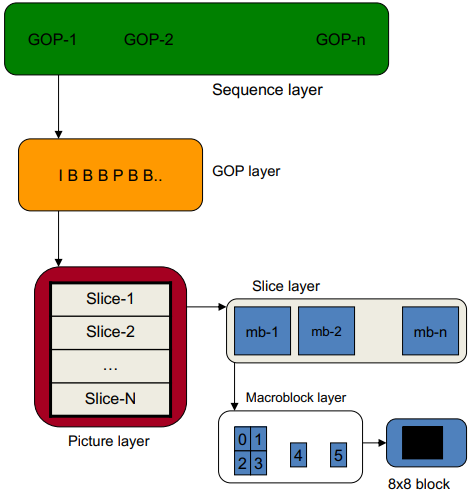
\includegraphics[width=\linewidth]{Bitstream structure.png}
\end{minipage}

\subsubsection{GOP - Group of Pictures}
Una sequenza video viene scomposta in gruppi di immagini (GOPs), dove GOP è la distanza tra due frame chiave. I frame possono essere di diversi tipi: 
\begin{itemize}
\item I (intra-coded): sono fotogrammi completi, identici ad un'immagine JPEG, e sono anche detti keyframes; si chiamano così perché vengono decodificati in modo indipendente dagli altri frame, minimizzando quindi gli errori e permettendo l'accesso random. La loro compressione è veloce ma produce file grandi.
\item P (predictive): sono codificati con previsioni di movimento rispetto ai frame I e P precedenti, migliorando quindi la compressione sfruttando la ridondanza temporale delle informazioni; memorizzano queste differenze usando dei motion vectors.
\item B (bi-directional): sono codificati con previsioni di movimento rispetto ai frame I e P precedenti e futuri; il movimento è dedotto mediante la media delle previsioni passate e future, il che li rende computazionalmente complessi e lenti da codificare.
\item D: contengono i coefficienti DC, usati solo nelle anteprime
\end{itemize}
\begin{figure} [h]
\centering
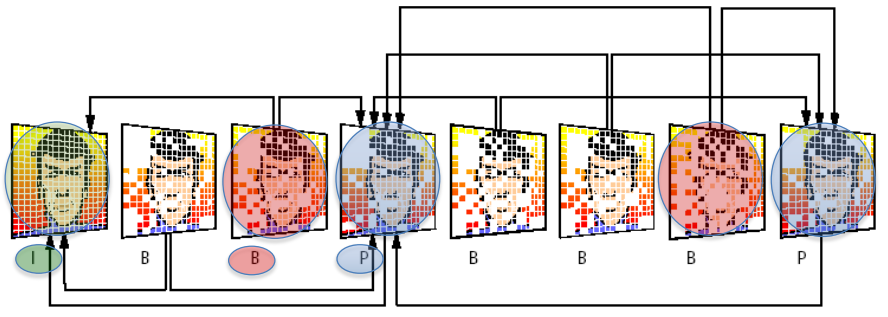
\includegraphics[width=0.8\textwidth]{IPB frames}
\end{figure}

Un GOP si dice chiuso se è possibile decodificarlo completamente senza bisogno di informazioni da altri GOP precedenti/successivi.\\
A parità di bitrate desiderato, un GOP più grande consente di comprimere più efficientemente e mantenere più dettagli nei frame. Questo però potrebbe far propagare per troppo tempo gli errori, che potrebbero diventare troppo evidenti: aggiungere quindi dei frame I può migliorare la resilienza agli errori, pur diminuendo la compressione totale. 

\subsubsection{Macroblocks}
Ogni frame video è diviso in macroblocchi (la più piccola unità indipendente considerata dall'MPEG), ovvero dei set di $16\times16$ pixel, che vengono usati per utilizzare i motion vector e gli error block. Ne esistono di 3 tipi:

\vspace{0.5em}
\noindent

\begin{minipage}{0.6\textwidth}
\begin{itemize}
\item Macroblock I: codificati indipendentemente dagli altri macroblock
\item Macroblock P: codificano il motion vector e l'error block del frame precedente (forward predicted macroblock)
\item Macroblock B: codificano il motion vector e l'error block del frame precedente e successivo (forward/backward predicted macroblock)
\end{itemize}
\end{minipage}
\hspace{0.05\textwidth} % Spazio bianco orizzontale tra le due minipage
\begin{minipage}{0.4\textwidth}
\centering
    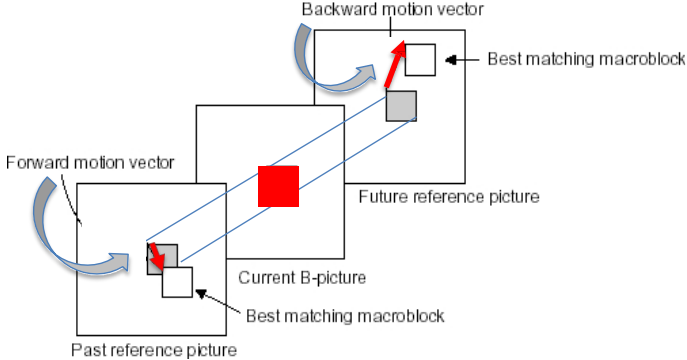
\includegraphics[width=0.9\linewidth]{Macroblocks.png}
\end{minipage}

\vspace{0.5em} 

I frame I e D, contenendo l'intera immagine, sono fatti di soli macroblock I; i frame P sono fatti di macroblock I o P; i frame B sono fatti di macroblock I, P o B.

\subsubsection{Macroblock Encoding}
\begin{center}
    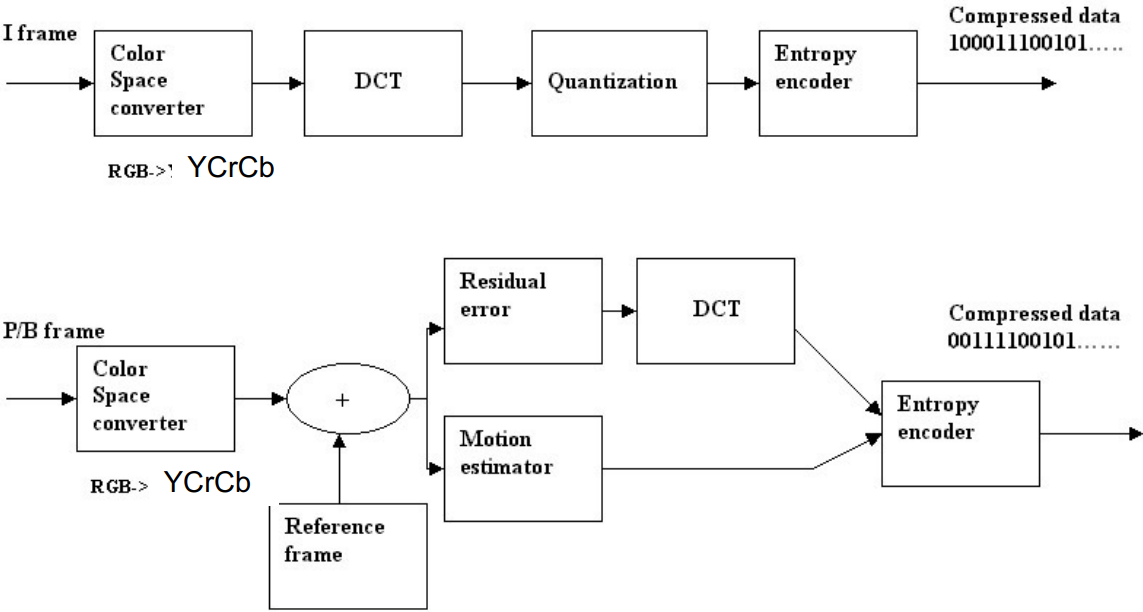
\includegraphics[width=0.64\linewidth]{Macroblock encoding.png}
\end{center}
\begin{itemize}
\item Block motion compensation: processo di sostituzione dei blocchi con un motion vector e un error block.
\item Motion vector: descrive la differenza tra blocchi simili in frame adiacenti; vengono infatti specificate 2 componenti (offset orizzontale e verticale). I motion vector vengono resettati quando si trova un nuovo macroblock I.
\item Error block: è un blocco ottenuto come differenza tra due motion compensated block
\end{itemize}

\subsubsection{Motion Estimation}
La motion estimation (stima del moto) è fatta attraverso algoritmi di block matching, che utilizzano diversi criteri tra loro:
\begin{itemize}
\item Mean Squared Error (MSE) $= \frac{1}{N^2} \sum_{ij} (C_{ij} - R_{ij})^2$
\item Sum of Squared Differences (SSD) $= \sum_{ij} (C_{ij} - R_{ij})^2$
\item Mean Absolute Error (MAE) $= \frac{1}{N^2} \sum_{ij} |C_{ij} - R_{ij}|$
\item Sum of Absolute Differences (SAD) $= \sum_{ij} |C_{ij} - R_{ij}|$
\item Matching Pel Count (MPC)
\end{itemize}
La SSD è più sensibile agli outliers (valori molto diversi) rispetto alla SAD.

\subsubsection{Search Matching Techniques}
Vengono utilizzate per trovare la miglior corrispondenza tra un blocco di riferimento e gli altri blocchi, utilizzando le formule scritte sopra.
\begin{itemize}
\item Full search technique: trova sempre il minimo globale, ma controllando tutte le posizioni (computazionalmente complesso)
\item Three step search (TSS, tipo ricerca binaria): complessità e performance basse
\item Logarithmic search: complessità e performance basse
\item One-ad-a-Time search: complessità e performance basse
\item Nearest Neighbours search: complessità moderata, ma buone performance
\end{itemize}

In alcuni casi la corrispondenza è migliorata se la ricerca viene eseguita su regioni generate artificialmente interpolando i pixel della regione originaria (sub-pixel)

\subsubsection{MPEG1 Encoder}
\begin{center}
    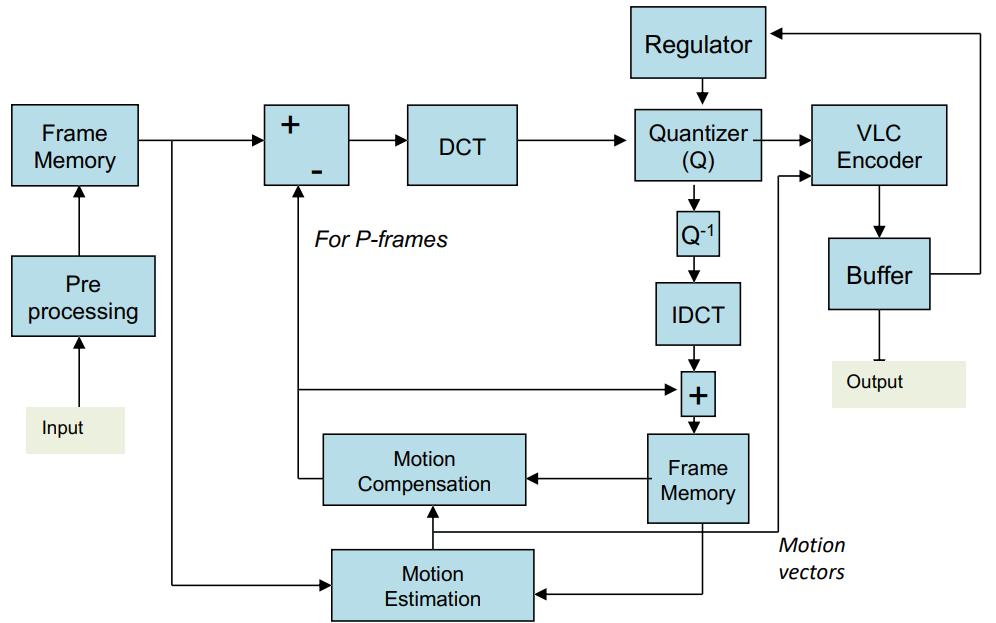
\includegraphics[width=0.8\linewidth]{MPEG1 encoder.png}
\end{center}

\subsection{MPEG-2, MPEG-4 H.264, MPEG-4 H.265}
Le fondamenta su cui si basano MPEG-1 e gli MPEG successivi sono più o meno simili, basandosi sui principi fondamentali di compressione video visti in precedenza. Le principali differenze fra MPEG-1 e gli MPEG successivi includono l'implementazione di tecniche di compressione più avanzate, che supportano una maggiore qualità video, risoluzione più alta, miglior gestione del movimento e l'introduzione di nuove funzionalità come la codifica a livelli di oggetti e la trasmissione su reti a larga banda.























\end{document}